% Chapter 1
%\newcommand {\DF}[2]{{\displaystyle\frac{#1}{#2}}}
\chapter{Tunnelling Spectroscopy with Proximity Effect} % Write in your own chapter title
\label{Chapter3}
\lhead{Chapter 3. \emph{Tunnelling Spectroscopy with Proximity Effect}} % Write in your own chapter title to set the page header

It is interesting to propose a theory calculating the $d$-wave conductance accounting for the proximity effect as required by our novel experiments. In this chapter, we limit our discussion to $s$-wave and $d_{x^2-y^2}$ cases.

Identical to the steps mentioned in the last chapter. We first solve the Bogoliubov equations and study the properties of the the tunnelling conductance kernel, $\sigma_S$ in (2.25). Then the knowledge of the conductance kernel, $\sigma_S$ will guide us to the desired $d$-wave proximity conductance.
Currently this work is in progress.
\section{Bogoliubov Equations}
As a matter of fact, the tunnelling conductance discussed in the previous chapter is based on a specific case which is shown in Fig.2.2. The potential is assumed as a $\delta$ function and the pair potential is assumed as a step function, so that Bogoliubov  equations(3.1) have an analytic solution. In contrast, such analytic solution no longer exists when dealing with more complicated case accounting for proximity effect where the gap is not simply a step function.
\subsection{Simplification for the Bogoliubov Equations}
The general Bogoliubov equations are 
\begin{eqnarray}\label{eq:GeneralBDG}
i\hbar\frac{\partial f}{\partial t} = \Big(-\frac{\hbar^2}{2m}\frac{\partial^2}{\partial {z^2}}-\mu(z)+V(z)\Big)f(z,t)+\Delta(z)g(z,t)\nonumber\\
\\
i\hbar\frac{\partial g}{\partial t} = \Big(-\frac{\hbar^2}{2m}\frac{\partial^2}{\partial {z^2}}-\mu(z)+V(z)\Big)g(z,t)+\Delta(z)f(z,t)\nonumber
\end{eqnarray}
Here we set $z$ as our tunnelling axis.
\eqref{eq:GeneralBDG} has the solution form 
\begin{eqnarray}
\varphi(z,t)=
\left(\begin{array}{c}
f(z,t)\\
g(z,t)
\end{array}\right)
\end{eqnarray}
where $\mu(z),\Delta(z),V(z)$ are chemical potential, energy gap, and the ordinary potential which is related to the barrier height, in which we are interested in the latter two.
By introducing a solution of the form in terms of the wave vector
\begin{eqnarray}\label{eq:wavefront}
f=u(z)e^{i\mathbf{k}_F\cdot\mathbf{z}-\frac{iEt}{\hbar}}\nonumber\\
\\
g=v(z)e^{i\mathbf{k}_F\cdot\mathbf{z}-\frac{iEt}{\hbar}}\nonumber\
\end{eqnarray}
$\mathbf{z}$ is the tunnelling axis vector. And $\mathbf{k_F}$ represents the fermi vector, whose amplitude $k_F$ is a CONSTANT for $d_{x^2-y^2}$-wave case and $s$-wave case. And we relate it to the coherence length, another CONSTANT.
\begin{eqnarray}\label{fermi vector}
\xi_0=\hbar v_F/(\pi\Delta_0)=\hbar^2k_F/(\pi m \Delta_0)
\end{eqnarray}
The term $\Delta_0$ is used in the expression \eqref{energy gap k and z} for $s$-wave and $d_{x^2-y^2}$ cases
\begin{eqnarray}\label{energy gap k and z}
&&\Delta(\mathbf{k},z)=\Delta_0\Delta(z)\Delta(\mathbf{k})\nonumber\\
&&\left.\Delta(z)\right|_{z=+\infty}=1,\left.\Delta(z)\right|_{z=-\infty}=0
\end{eqnarray}
We also define the following function for convenience
\begin{eqnarray}\label{delta infty}
\Delta_{\infty}=\Delta(\mathbf{k},+\infty)=\Delta(\mathbf{k})
\end{eqnarray}
The Bogoliubov equations could be written in this way neglecting higher order terms\citep{Reference4}.
\begin{eqnarray}\label{eq:BdG}
&&\DF{\partial u}{\partial z}=i(\pi \xi_0\Delta_0\cdot(\widehat{\mathbf{k}}\cdot\widehat{\mathbf{z}}))^{-1}[Eu-\Delta(z)v]\nonumber\\
&&\DF{\partial v}{\partial z}=-i(\pi \xi_0\Delta_0\cdot(\widehat{\mathbf{k}}\cdot\widehat{\mathbf{z}}))^{-1}[Ev-\Delta(z)u]\nonumber\\
&&\widehat{\mathbf{k}}=\frac{\mathbf{k}}{|\mathbf{k}|},\widehat{\mathbf{z}}=\frac{\mathbf{z}}{|\mathbf{z}|}
\end{eqnarray}
which are the equations we are interested in, $\xi_0$ is the coherence length. Also we have the accompanied boundary conditions taking into account the potential $V(z)=Z_0(\pi\xi_0\Delta_0)\delta(z)$
\begin{eqnarray}\label{eq:OridinaryBoundary}
&&\left.\varphi\right|_{z=0^+}=\left.\varphi\right|_{z=0^-}\nonumber\\
\\
&&\left.\frac{\partial \varphi}{\partial z}\right|_{z=0^+}-\left.\frac{\partial \varphi}{\partial z}\right|_{z=0^-}=\left.2k_FZ_0\varphi\right|_{z=0^+}\nonumber
\end{eqnarray}

As indicated in the reference\citep{Reference4}, the Bogliubov equations are solved region by region, which finally lead us to the tunnelling conductance kernel. 
\begin{eqnarray}\label{sub-kernel}
\sigma_S=1+A-B
\end{eqnarray}
The andreev reflection $A$ and ordinary reflection $B$ in \eqref{sub-kernel} could be directly calculated from the solutions from the Bogliubov equations.

\subsection{Solving the Bogoliubov Equations}
We divide the tunnelling axis into four regions, named 'super','reduced','induced','normal', respectively, which is shown in Fig.3.1, where we already choose parabolic shape for the pair potential.
\begin{figure}[htbp]
\small
	\centering
		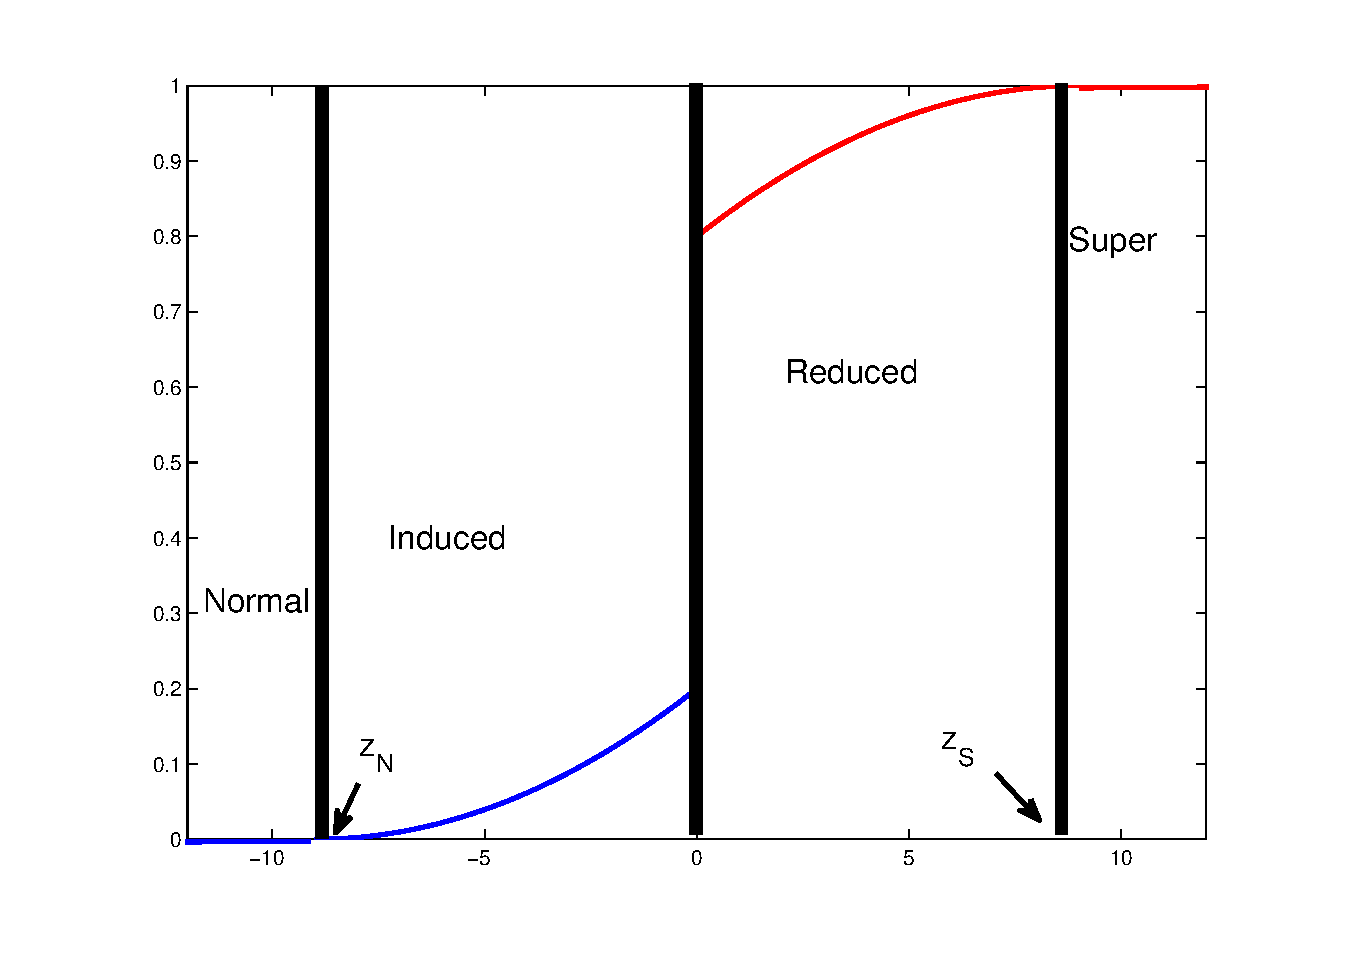
\includegraphics[width=10cm]{./Figures/3-2-1.eps}
		\rule{35em}{0.5pt}
	\caption[An Electron]{Parabolic shapes of reduced and induced pair potential. The tunnelling axis is divided into four regions.}
	\label{fig:EnergyGap}
\end{figure}
Now we solve the Bogoliubov equations region by region.

$\mathbf{\bullet \ 'Super'  \  Region}$

In the 'super' region, we already know the solution in \eqref{eq:superform}-\eqref{eq:superpara2}.
\begin{eqnarray}\label{eq:superform}
&&\varphi_1=
\left(
\begin{array}{c}
 u_0\\
 v_0
 \end{array}\right)e^{i(\mathbf{k}_F+\mathbf{k}'_S)\cdot\mathbf{z}}\nonumber\\
&&\\
&&\varphi_2=
\left(
\begin{array}{c}
 v_0\\
 u_0
 \end{array}\right)e^{-i(\mathbf{k}_F-\mathbf{k}'_S)\cdot\mathbf{z}}\nonumber
\end{eqnarray}
where parameters are already known,
\begin{eqnarray}\label{eq:superpara1}
u_0^2=1-v_0^2=\frac{1}{2}\Big(1+\frac{(E^2-\Delta_{\infty}^2)^{\frac{1}{2}}}{E}\Big)
\end{eqnarray}
where $\Delta_{\infty}$ is defined in \eqref{delta infty} and 
\begin{eqnarray}\label{eq:superpara2}
k_S'=k_S/(\widehat{\mathbf{k}}\cdot\widehat{\mathbf{z}})=(E^2-\Delta_{\infty}^2)^{1/2}(\pi \xi_0 \Delta_0(\widehat{\mathbf{k}}\cdot\widehat{\mathbf{z}}))^{-1}
\end{eqnarray}
The solution of this region serves as the generator of boundary conditions \eqref{reduceboundary} for the solution of the next region,'reduced' by applying the continuity of the wave functions $\varphi$ and the derivative of the wave functions $\partial\varphi/\partial z$. 

$\mathbf{\bullet \ Reduced \ Region}$
The solution of reduced region is assumed to have the form \eqref{reducedform}.
\begin{eqnarray}\label{reducedform}
\varphi_j=
\left(
\begin{array}{c}
 u_{aj}\\
 v_{aj}
 \end{array}\right)e^{i\mathbf{k}_F\cdot\mathbf{z}}+
 \left(
\begin{array}{c}
 v_{bj}\\
 u_{bj}
 \end{array}\right)e^{-i \mathbf{k}_F\cdot\mathbf{z}},j=1,2
\end{eqnarray}
Realising that $\mathbf{k}'_S\cdot\mathbf{z}=k_S/\cos\theta\widehat{\mathbf{k}}\cdot\widehat{\mathbf{z}}=k_Sz$ according to \eqref{eq:superpara2}, the boundary condition for the reduced region is
\begin{eqnarray}\label{reduceboundary}
&&u_{a1}(z_S)=u_{b2}(z_S)=u_0 e^{ik_Sz_S}\nonumber\\
&&v_{a1}(z_S)=v_{b2}(z_S)=v_0 e^{ik_Sz_S}\nonumber\\
&&\\
&&u_{b1}(z_S)=u_{a2}(z_S)=0\nonumber\\
&&u_{b1}(z_S)=u_{a2}(z_S)=0\nonumber
\end{eqnarray}
The term $z_S$ and $z_N$ are shown in Fig.\ref{fig:EnergyGap} and indicate the boundary of the reduced region with the super region and the normal region with the induced region respectively.
After obtaining the numerical solutions for \eqref{reducedform}, we select the values of only one point, which is at $z=0$
\begin{eqnarray}
&&u_{a1}(0)=u_{b2}(0)=u_{a1}^+\nonumber\\
\\
&&v_{a1}(0)=v_{b2}(0)=v_{a1}^+\nonumber
\end{eqnarray}
Before we move to the induced region, we make use of the original boundary condition at $z=0$, setting $V(z)=Z_0(\pi\xi_0\Delta_0)\delta(z)$.  In the boundary conditions \eqref{0condition}, the symbols $+,-$ represent $z=0^+,z=0^-$, respectively.
\begin{eqnarray}\label{0condition}
&&\left.\varphi\right|_{z=0^+}=\left.\varphi\right|_{z=0^-}\nonumber\\
\\
&&\left.\frac{\partial \varphi}{\partial z}\right|_{z=0^+}-\left.\frac{\partial \varphi}{\partial z}\right|_{z=0^-}=\left.2k_FZ_0\varphi\right|_{z=0^+}\nonumber
\end{eqnarray}
We neglect terms $u_{b1}(z), u_{a2}(z), v_{b1}(z), v_{a2}(z)$as they are zero because they have $0$ initial values in \eqref{reduceboundary}. 

$\mathbf{\bullet \ Induced \ Region}$
In light of the boundary conditions \eqref{0condition}, we write the solution of the induced region in the form of
\begin{eqnarray}\label{induced form}
&&\varphi_1=
(1+iZ)\left(
\begin{array}{c}
 u_{a0}\\
 v_{a0}
 \end{array}\right)e^{i\mathbf{k}_F\cdot\mathbf{z}}-iZ\left(
\begin{array}{c}
 v_{b0}\\
 u_{b0}
 \end{array}\right)e^{-i\mathbf{k}_F\cdot\mathbf{z}}\nonumber\\
&&\varphi_1=
iZ\left(
\begin{array}{c}
 u_{b0}\\
 v_{b0}
 \end{array}\right)e^{i\mathbf{k}_F\cdot\mathbf{z}}+(1-iZ)\left(
\begin{array}{c}
 v_{a0}\\
 u_{a0}
 \end{array}\right)e^{-i\mathbf{k}_F\cdot\mathbf{z}}\nonumber\\
 &&Z=\frac{Z_0}{\widehat{\mathbf{k}}\cdot\widehat{\mathbf{z}}}
\end{eqnarray}

Then the boundary conditions for the induced region are expressed in \eqref{inducedboundary}.
\begin{eqnarray}\label{inducedboundary}
u_{a0}^-=u_{a1}^+,v_{a0}^-=v_{a1}^+\nonumber\\
\\
u_{b0}^-=v_{a1}^+,v_{b0}^-=u_{a1}^+\nonumber
\end{eqnarray}

$\mathbf{\bullet \ Normal \ Region}$
After the induced solution is numerically obtained, we again choose the value only at $z=-z_N$, which is the interface of induced region and normal region.
\begin{eqnarray}\label{normal condition}
u_a=u_{a0}(-z_N),v_a=v_{a0}(-z_N)\nonumber\\
\\
u_b=u_{b0}(-z_N),v_b=u_{b0}(-z_N)\nonumber
\end{eqnarray}

The solution in the normal region has the form \eqref{normal form}, noting that we already make wave vectors parallel to the incident.
\begin{eqnarray}\label{normal form}
\varphi_j=\nu_j\Big[
\left(
\begin{array}{c}
1\\
0
\end{array}\right)e^{i(k_F+k_N)z}+a_e\left(
\begin{array}{c}
0\\
1
\end{array}\right)e^{i(k_F-k_N)z}+b_e\left(
\begin{array}{c}
1\\
0
\end{array}\right)e^{-i(k_F+k_N)z}\Big]\nonumber\\
+\eta_j\Big[
\left(
\begin{array}{c}
0\\
1
\end{array}\right)e^{-i(k_F-k_N)z}+a_h\left(
\begin{array}{c}
1\\
0
\end{array}\right)e^{-i(k_F+k_N)z}+b_h\left(
\begin{array}{c}
0\\
1
\end{array}\right)e^{i(k_F-k_N)z}\Big]
\end{eqnarray}
The coefficients in (3.17) could again be obtained by applying the the continuity.
\begin{eqnarray}\label{reflection terms}
&&a_e=\frac{(1+Z^2)u_av_a-Z^2u_bv_b}{(1+Z^2)u_a^2-Z^2u_b^2}e^{-2ik_Nz_N}\nonumber\\
&&\\
&&b_e=\frac{iZ(1-iZ)(u_bv_a-u_av_b)}{(1+Z^2)u_a^2-Z^2u_b^2}e^{-2ik_Nz_N}\nonumber
\end{eqnarray}
So that the tunnelling conductance kernel versus energy is written as 
\begin{eqnarray}
\sigma_S=1+A-B=1+\left\vert a_e\right\vert^2-\left\vert b_e\right\vert^2
\end{eqnarray}



\section{Properties of Tunnelling Spectroscopy Kernel with Proximity Effect at Normal Incident}
Under the condition of the normal incident, $\widehat{\mathbf{k}}\cdot\widehat{\mathbf{z}}=1$. 

\subsection{The Shapes of Reduced and Induced Pair Potential}
To be precise we need to compute the pair potential using self-consistent method\citep{Reference11}. Yet we won't lose two much information if we only guess the shape of the pair potential\citep{Reference8, Reference4}. We are using parabolic shape of pair potential which is like Fig.\ref{fig:EnergyGap}

Another point we should account for is the proximity thickness, which will affect much the shape of the computed results. We define
\begin{eqnarray}
z_S=a_S\pi\xi_0,z_N=a_N\pi\xi_0,\xi_0=\hbar^2k_F/(\pi m\Delta_0)
\end{eqnarray}
where in effect we find the factors $a_S,a_N$ play the role of influencing the results.
Therefore, we choose the potential function as 
\begin{eqnarray}\label{spatial form of gap}
&&\Delta_R(\mathbf{k},z)=\frac{\Delta_r(\mathbf{k})-\Delta_{\infty}}{z_S^2}(z-z_S)^2+\Delta_{\infty}(\mathbf{k})\nonumber\\
&&\\
&&\Delta_I(\mathbf{k},z)=\frac{\Delta_i(\mathbf{k})}{z_N^2}(z+z_S)^2\nonumber
\end{eqnarray}
who have the shapes in \ref{fig:EnergyGap}. The terms $\Delta_r,\Delta_i$ represents the reduced gap and induced gap, respectively. Since it is in $s$-wave in the current discussion, the terms appearing in \eqref{spatial form of gap} are all independent of $\mathbf{k}$ space.

\subsection{Specific Cases}
We check the reliability of our model by calculating the specific cases of the tunnelling kernel\eqref{sub-kernel}. In the following we set $\Delta_0=1$ in \eqref{energy gap k and z}.

First, BTK is a special case of proximity effect; in other words, if we set $\Delta_R=1,\Delta_I=0$, we should see the results of BTK, Fig.\ref{fig:BTK reproduction}. Fig.\ref{fig:BTK reproduction} compares the plots generated from the formula \eqref{1DKernel} and from solving the Bogoliubov equations discussed in the last section. We calculate the tunnelling conductance for various barrier nights and see the two results match quite well. 
\begin{figure}[htbp]
\small
	\centering
		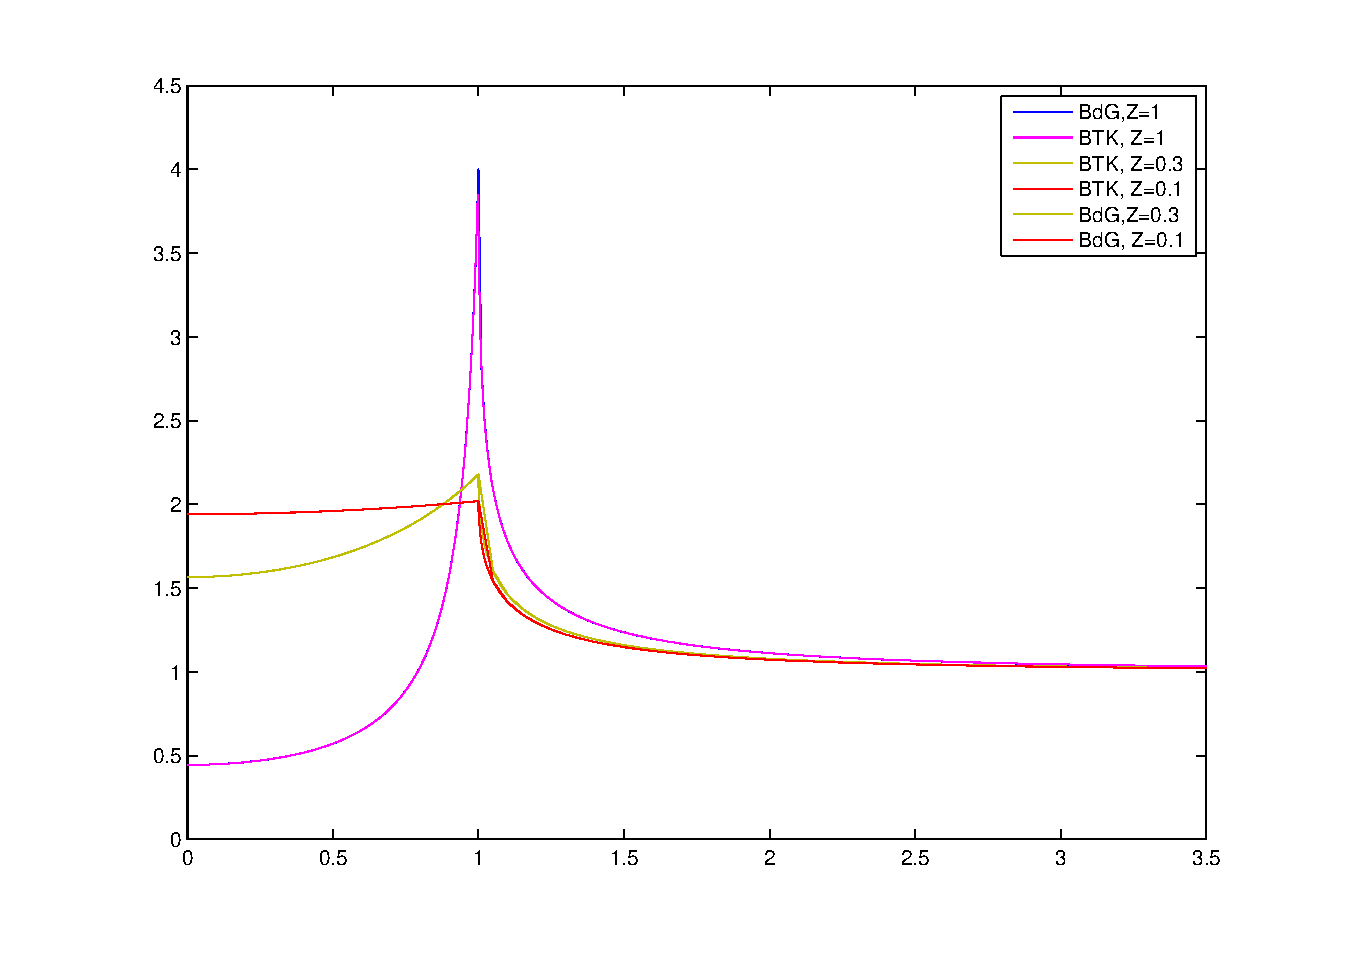
\includegraphics[width=10cm]{./Figures/3-2-8.eps}
		\rule{35em}{0.5pt}
	\caption[An Electron]{BTK case when we set $\Delta_R=1,\Delta_I=0$}
	\label{fig:BTK reproduction}
\end{figure}

Also, when barrier height $Z_0=0$, we should observe flat region with the value of $2$ in the middle, Fig.\ref{fig:z reproduction}.
\begin{figure}[htbp]
\small
	\centering
		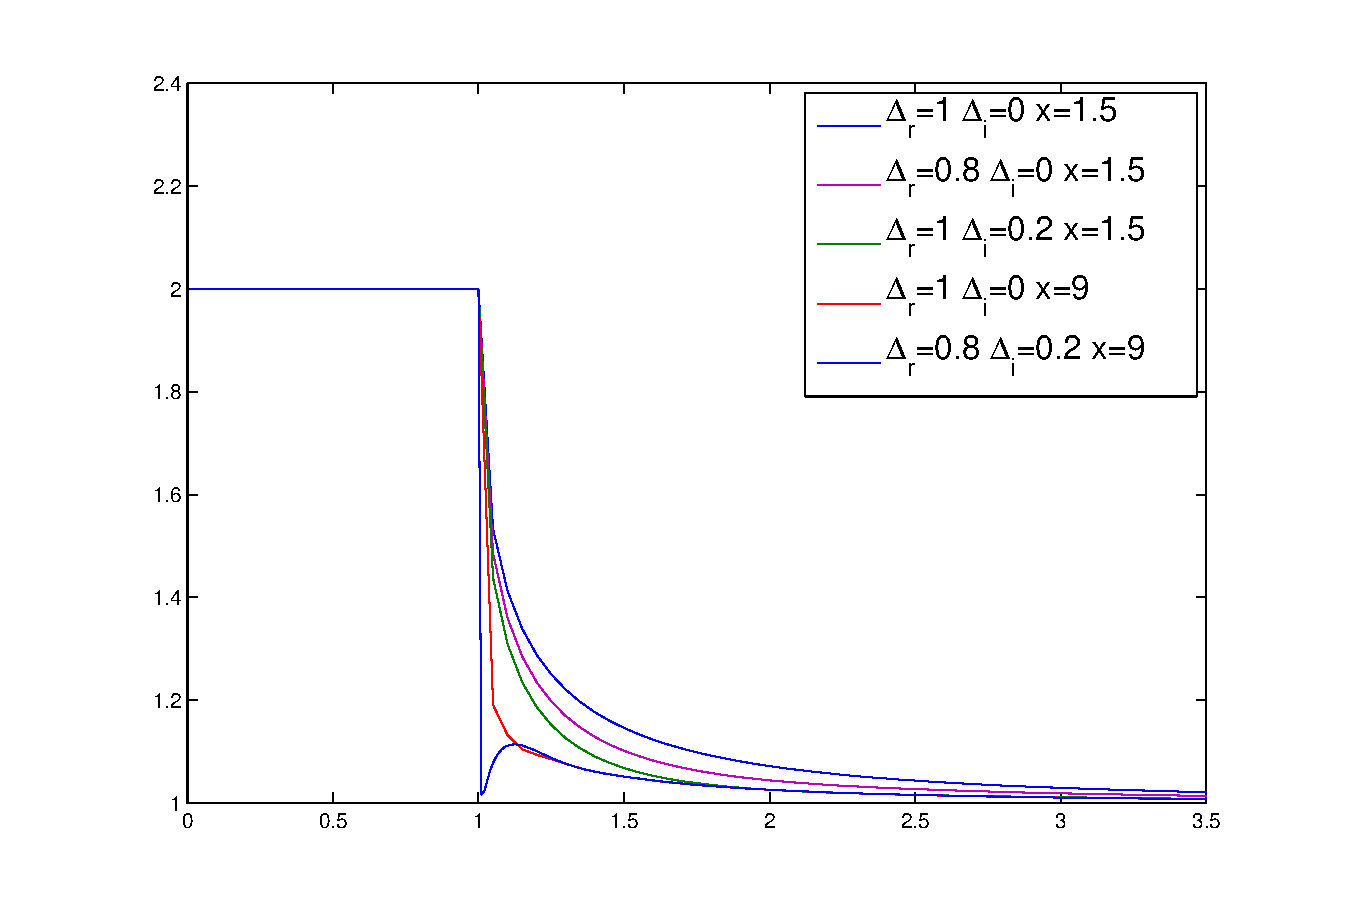
\includegraphics[width=10cm]{./Figures/3-2-9.eps}
		\rule{35em}{0.5pt}
	\caption[An Electron]{The flat region in the middle appears no matter what reduced gap and induced gap and the proximity region thickness are}
	\label{fig:z reproduction}
\end{figure}

\subsection{$s$-wave Proximity Effect at Normal Incident with Various Parameters}
Similar to the procedure in the previous chapter, with solutions obtained, we first have a look at the kernel of the conductance,$\sigma_S$, in \eqref{sub-kernel}.

We draw a list of figures showing the change of the shape according to the varying reduced gap and induced gap, setting the coherence length as $\pi\xi_0=1$, Fig.\ref{Z=0.3reducedthin}-Fig.\ref{Z=0.3induced}.
\begin{figure}[htbp]
\small
\centering
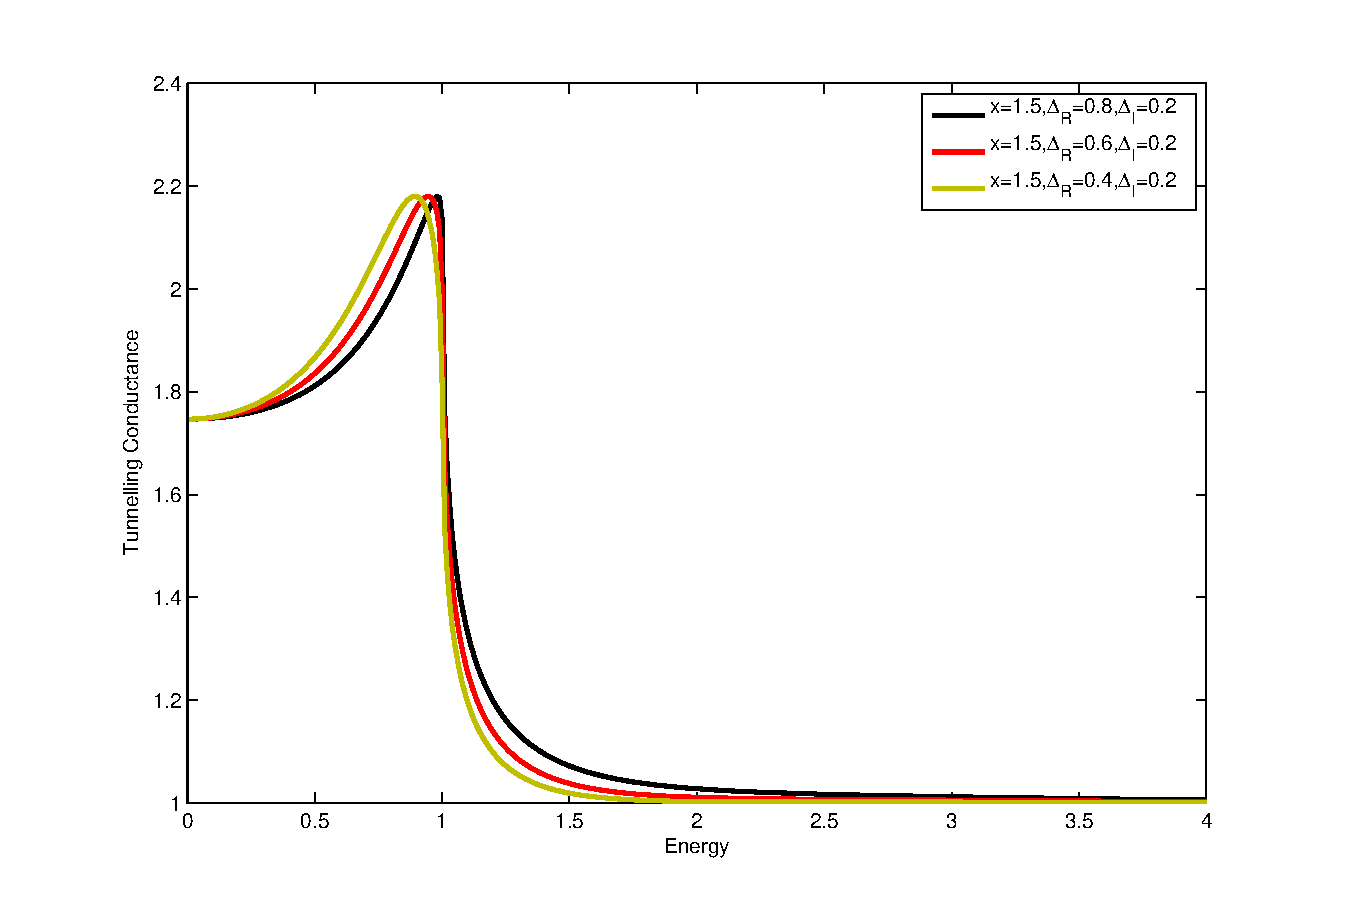
\includegraphics[width=10cm]{3-3-4.eps}
\caption{Low barrier height $Z_0=0.3$ for various values of the reduced gap. We don't see many peaks when the proximity region is thin.}
\label{Z=0.3reducedthin}
\end{figure} 
\begin{figure}[htbp]
\small
\centering
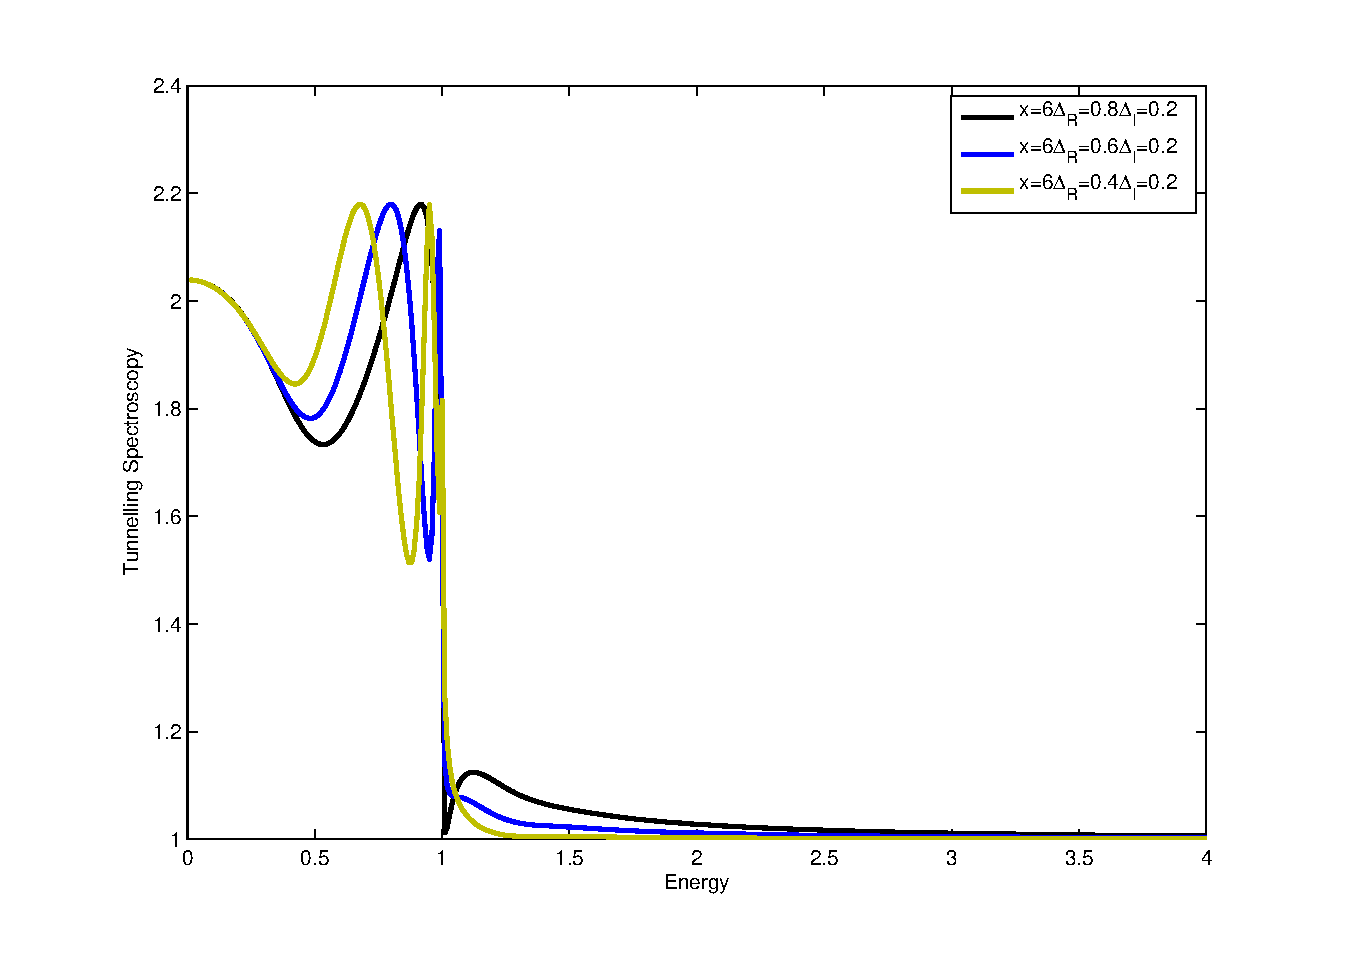
\includegraphics[width=10cm]{3-3-5.eps}
\caption{Some peaks show if thicker proximity region is chosen at low barrier height, with reduced gap varying and included gap fixed.$Z_0=0.3$.}
\label{Z=0.3reduced}
\end{figure}
\begin{figure}[htbp]
\small
\centering
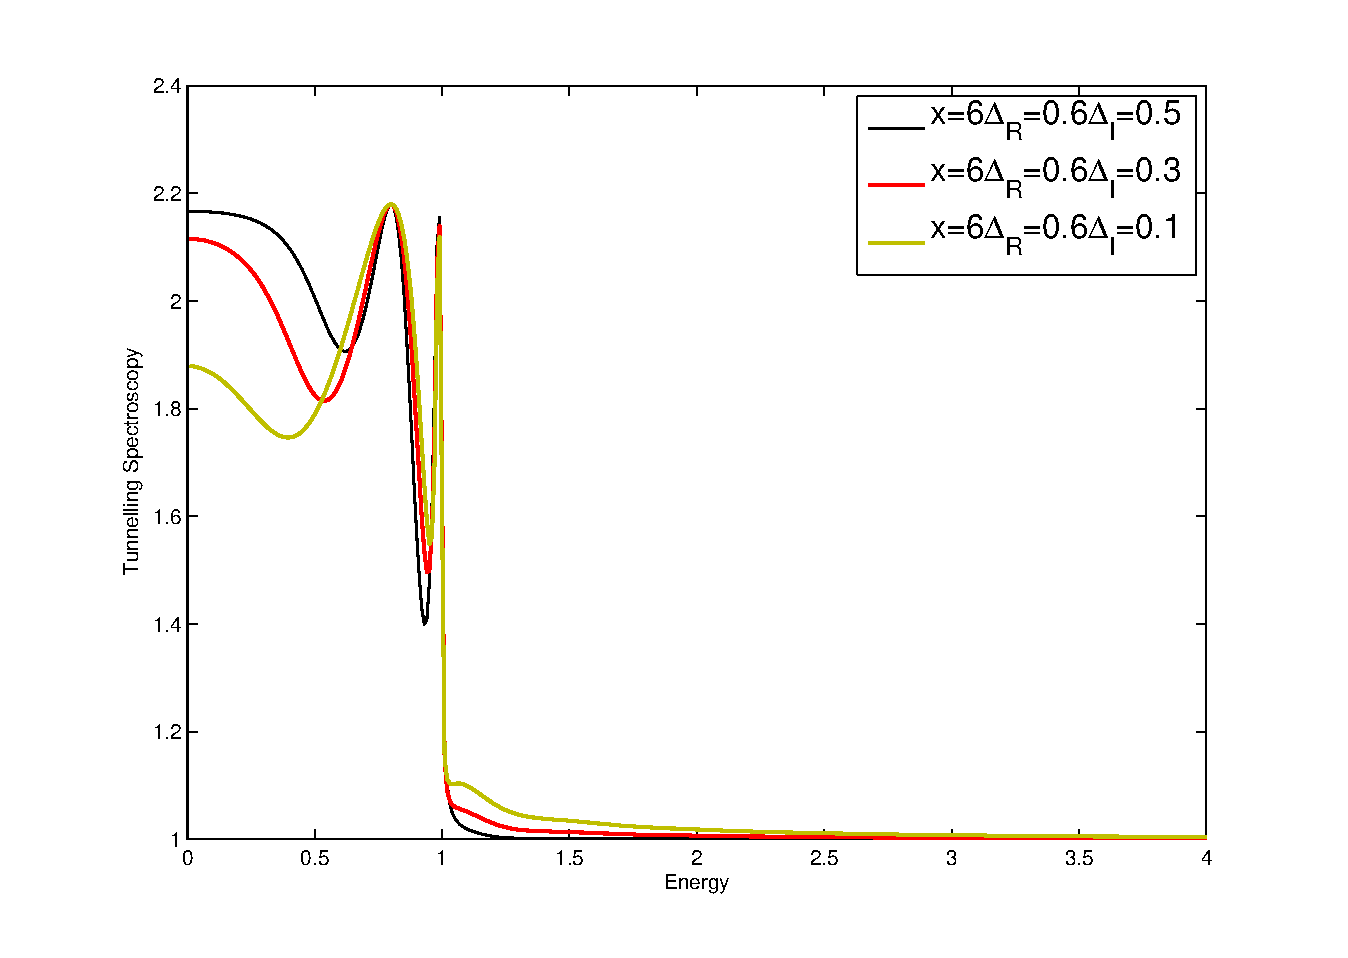
\includegraphics[width=10cm]{3-3-6.eps}
\caption{Some peaks show if thicker proximity region is chosen at low barrier height, with induced gap varying and reduced gap fixed.$Z_0=0.3$.}
\label{Z=0.3induced}
\end{figure}


\begin{comment}
\begin{figure}[htbp]
\small
\centering
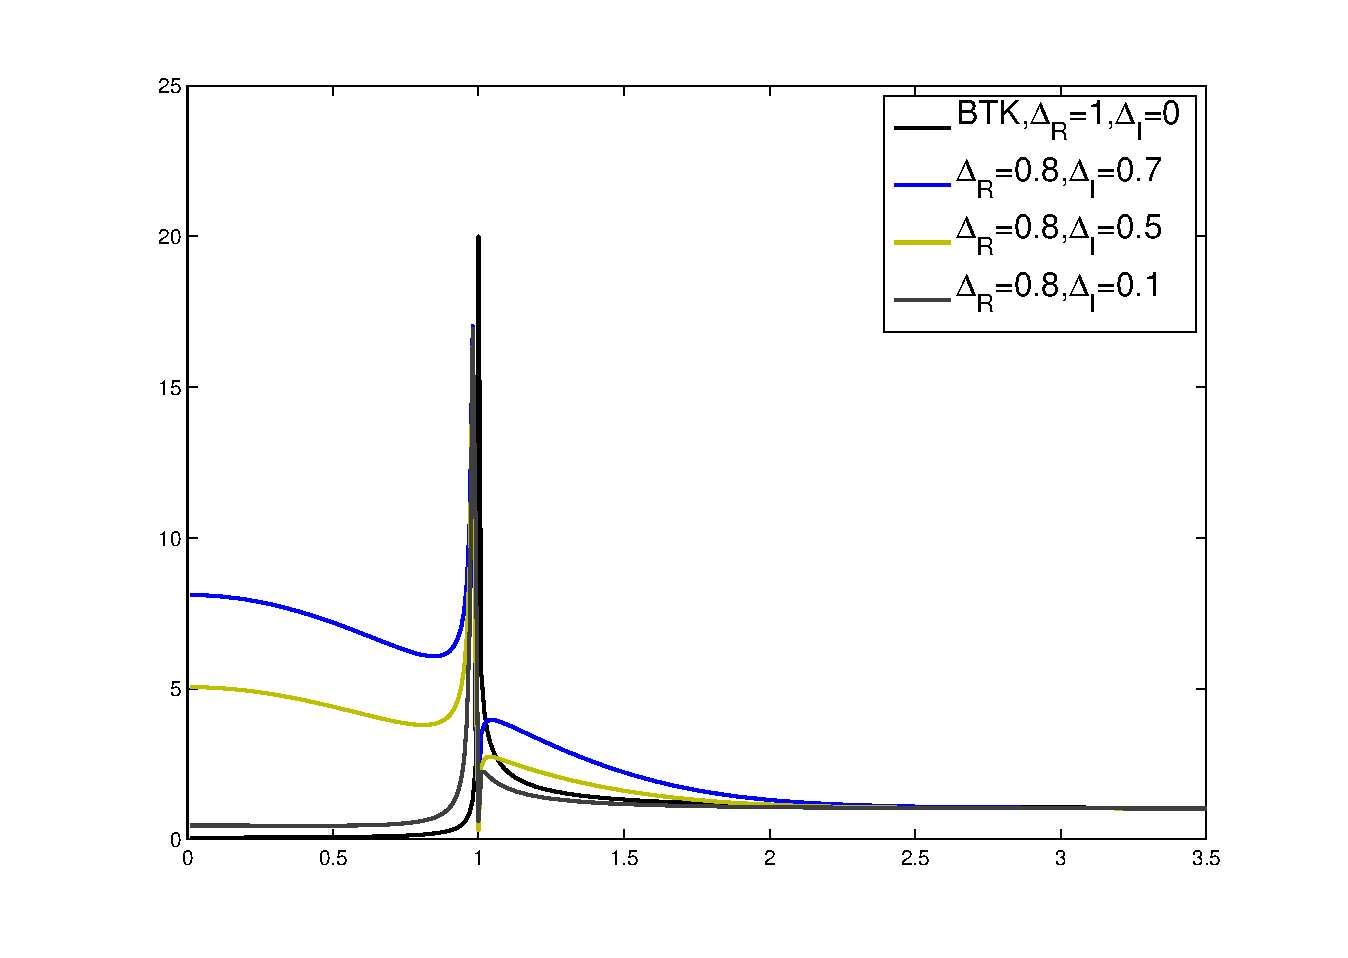
\includegraphics[width=10cm]{3-3-1.eps}
\caption{The figure indicates the difference with induced gap varying.$Z_0=0.3$.}
\label{Z=0.3induced}
\end{figure}
\begin{figure}[htbp]
\small
\centering
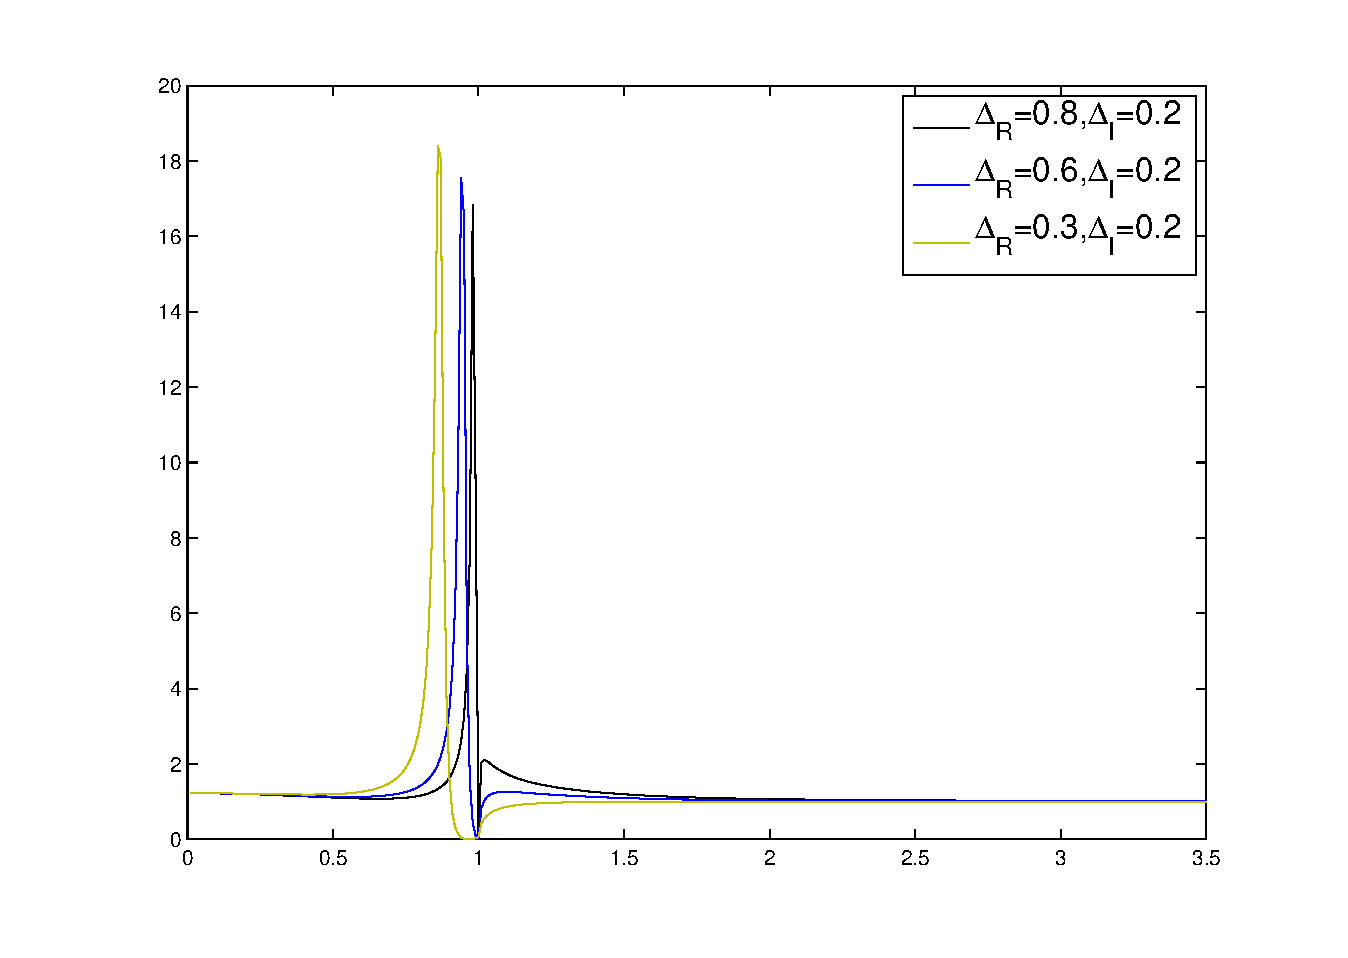
\includegraphics[width=10cm]{3-3-2.eps}
\caption{The figure indicates the difference with reduced gap varying.$Z_0=3$.}
\label{fig:6}
\end{figure}
\end{comment}

Also, as a thought, the proximity region width scaled on the coherence length may affect the transmission. Comparing the plots in Fig.\ref{fig:kernel x} or comparing Fig.\ref{Z=0.3reducedthin} with Fig.\ref{Z=0.3reduced}, we can discover the difference. The thicker proximity region leads to the higher conductance value close to $E=0$ and create more peaks.
\begin{figure}[htbp]
\small
\centering
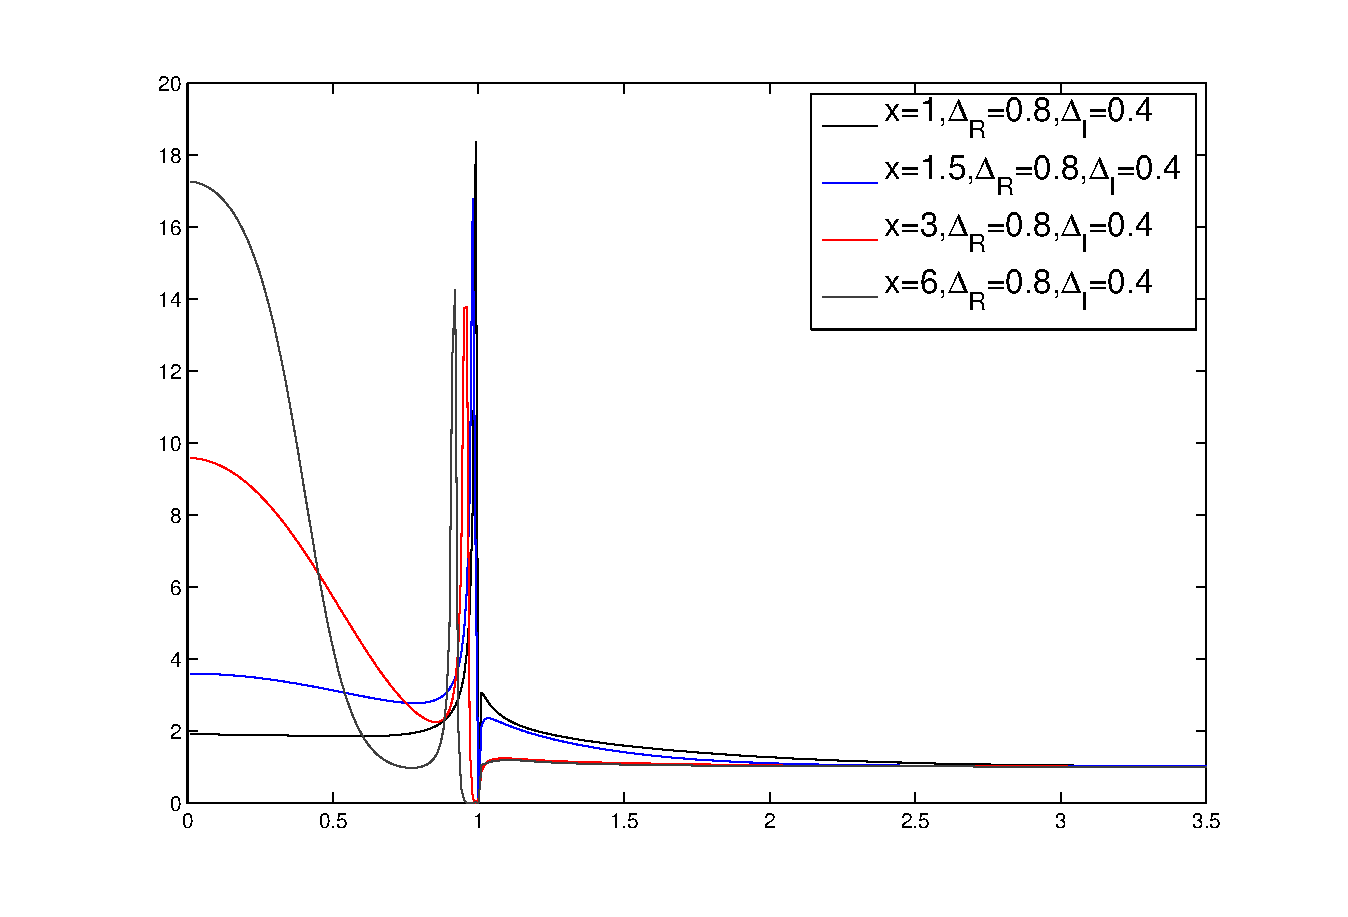
\includegraphics[width=10cm]{3-3-3.eps}
\caption{Increasing the proximity thickness leads to increasing value in the middle and create more peaks. $Z_0=3$}
\label{fig:kernel x}
\end{figure}

The Fig.\ref{MapInduced} and Fig.\ref{MapReduced} gives us a clearer picture of the existence of the reduced gap and induced gap.

In Fig.\ref{MapInduced}, we set bulk gap $\Delta_0=2$, fix the reduced gap $\Delta_r=1$ and vary the induced gap $\Delta_i$ from $0$ to $1.5$.  The red tongue in the middle indicates the properties of the varying induced gap, whose width is from $0$ to about $1.5$, corresponding to the value of induced gap at that point.
\begin{figure}[htbp]
\small
	\centering
		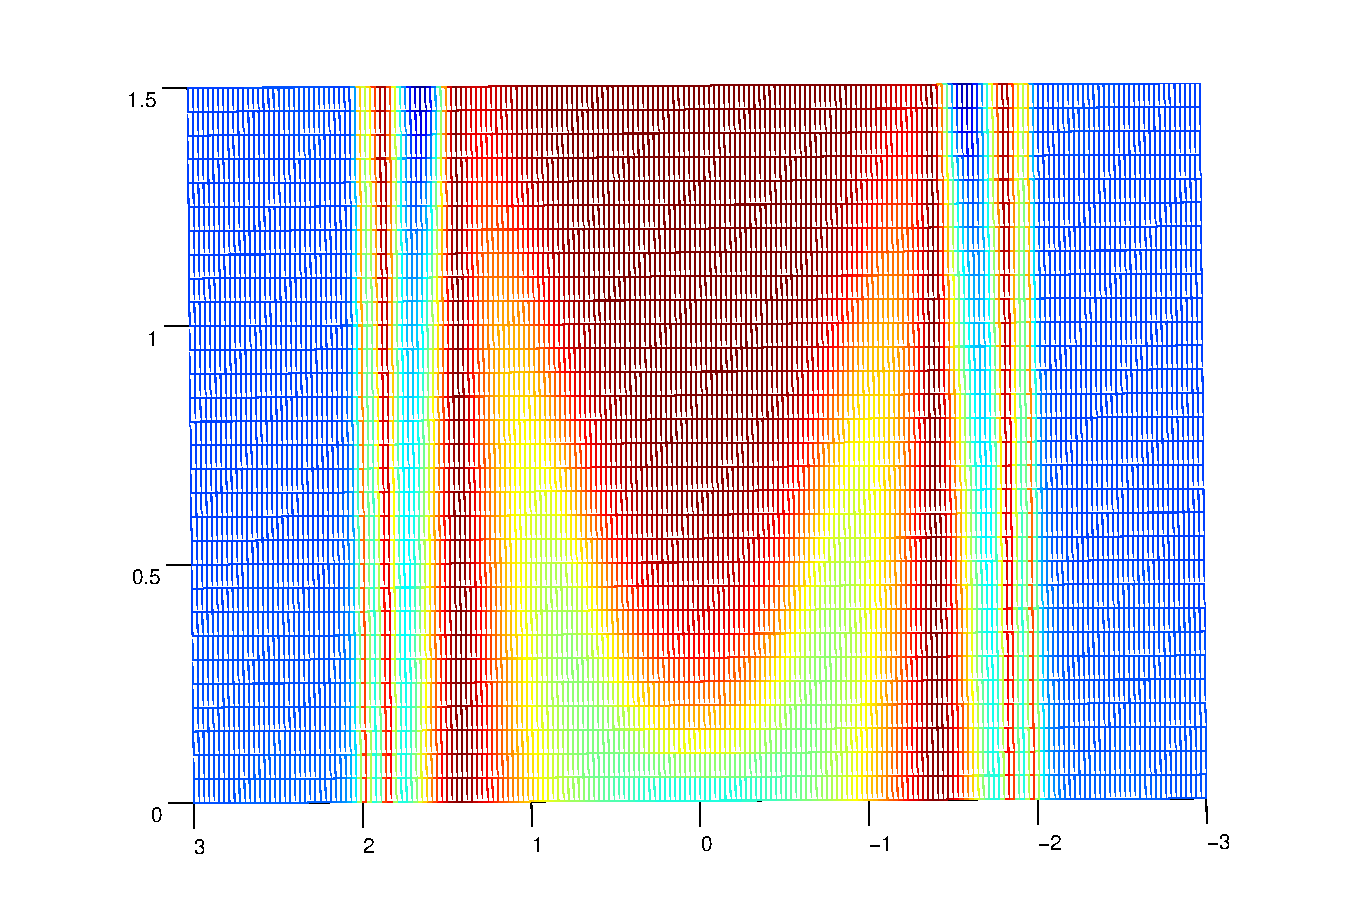
\includegraphics[width=10cm]{./Figures/3dinduce.eps}
		\rule{35em}{0.5pt}
	\caption[An Electron]{The picture shows the properties of the tunnelling conductance when induced gap is varying while reduced gap is fixed. The blue colour indicates the low conductance value while in contrast the red colour indicates the high conductance value.}
	\label{MapInduced}
\end{figure}

In Fig.\ref{MapReduced}, we set bulk gap $\Delta_0=2$, fix the induced gap $\Delta_i=0.4$ and vary the reduced gap $\Delta_r$ from $0$ to $2$.  The red rectangular with $width=0.8$ shows the existence of the induced gap. The two branches growing from the bottom indicates the existence of the reduced gap. The minimum value of the reduced gap in the bottom seems to be expelled by the induced gap that it could not reach $0$ as it should be. The maximum value of the reduced gap is at $1$ as it should be.
\begin{figure}[htbp]
\small
	\centering
		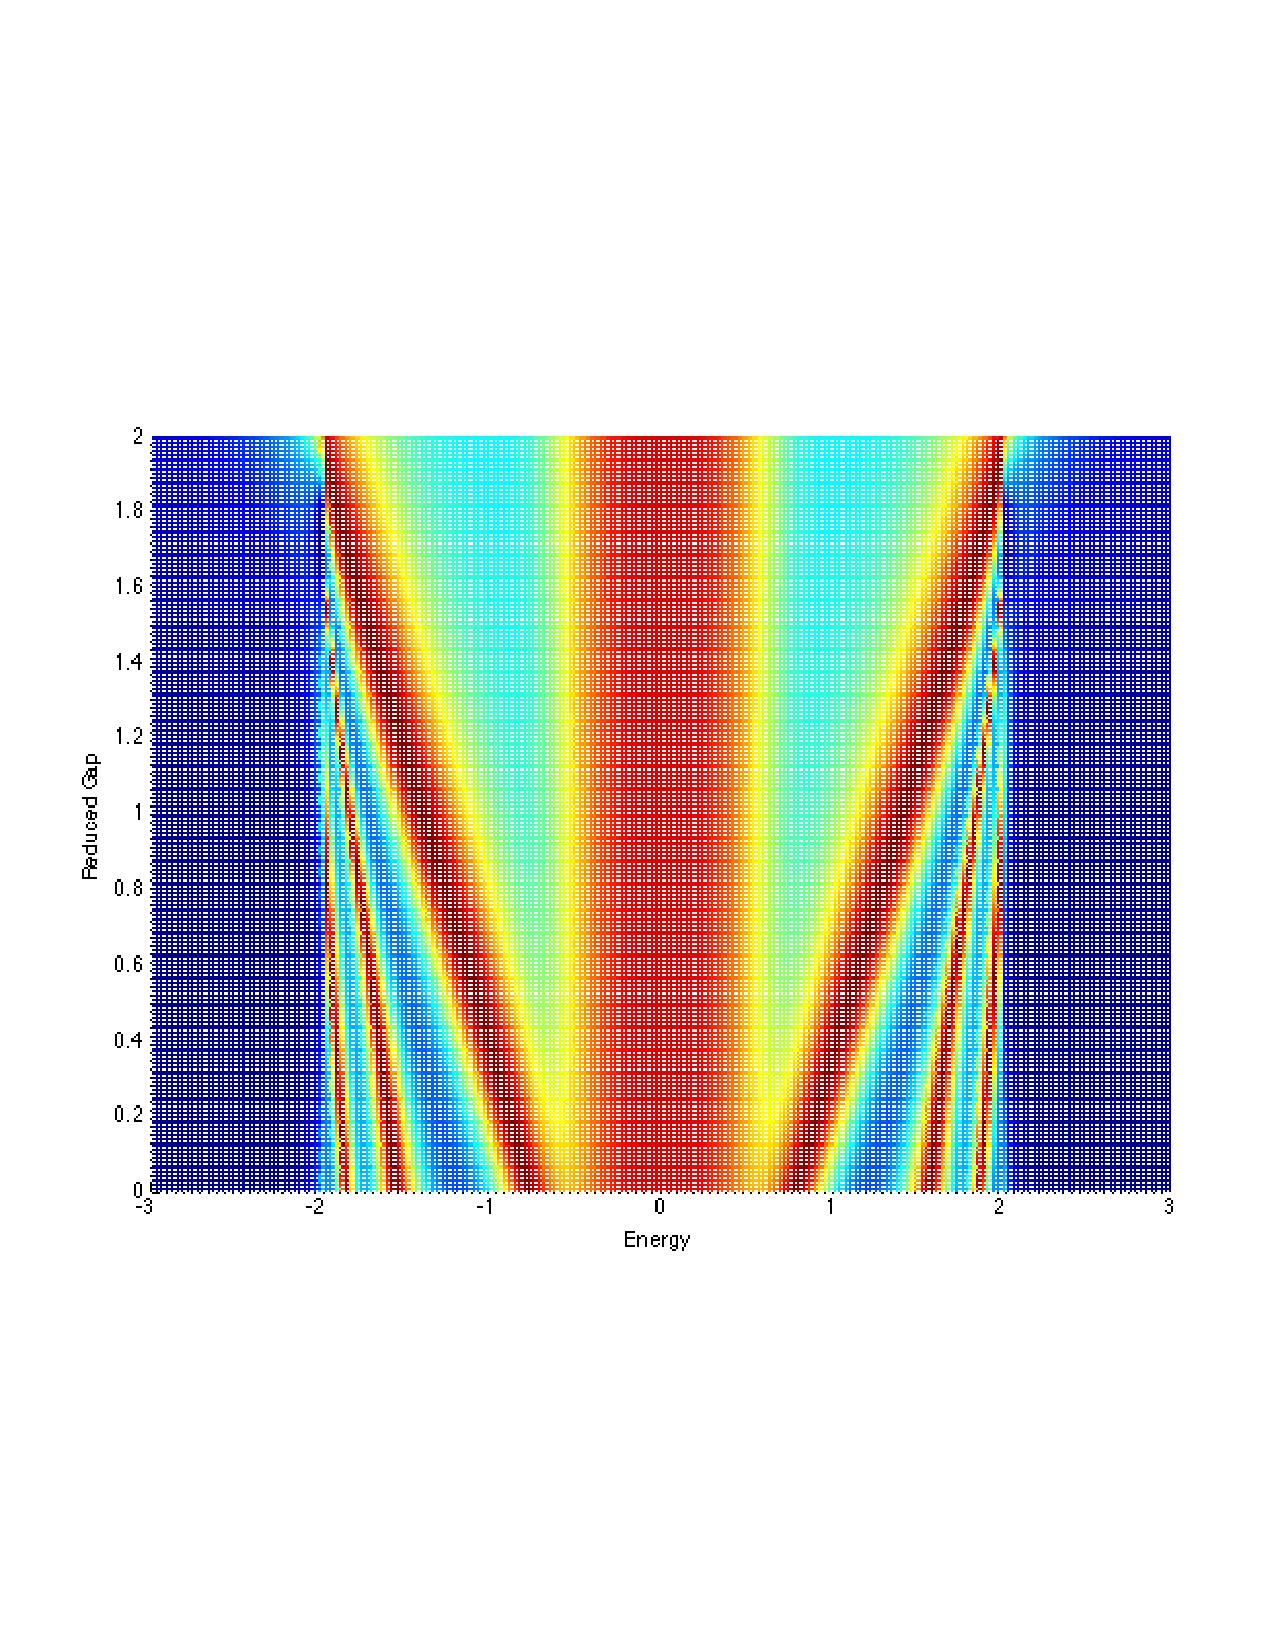
\includegraphics[width=12cm]{./Figures/3dreduceinduce.pdf}
		\rule{35em}{0.5pt}
	\caption[An Electron]{The picture shows the properties of the tunnelling conductance when the reduced gap is varying while the induced gap is fixed. The blue colour indicates the low conductance value while in contrast the red colour indicates the high conductance value.}
	\label{MapReduced}
\end{figure}
%%%%new section
\section{An In Progress Approach to the $d$-wave Tunnelling Spectroscopy with Proximity Effect}
\begin{figure}[htbp]
\small
	\centering
		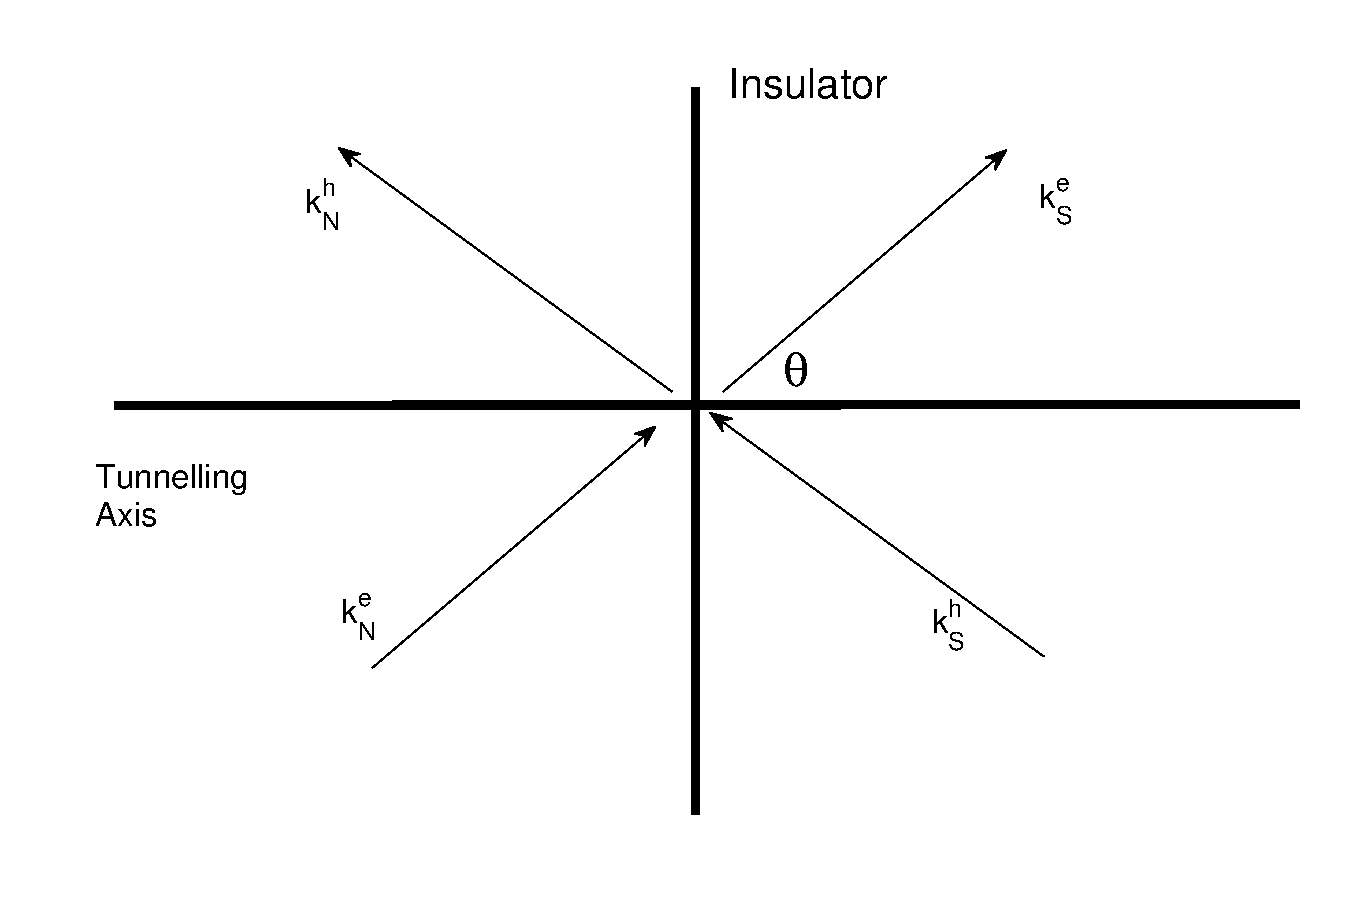
\includegraphics[width=10cm]{./Figures/3-5-1.eps}
		\rule{35em}{0.5pt}
	\caption[An Electron]{The four processes happen at the insulator. $k_S^e$ is the ordinary electron reflection vector;  $k_S^h$ is the hole reflection vector; $k_N^e$ is the electron transmission vector; $k_S^h$ is the hole transmission vector.}
	\label{fig:Andreev}
\end{figure}
In the $d$-wave tunnelling case, the transmission and reflection is interpreted in Fig~\ref{fig:Andreev}.  Note that the wave-vector parallel to the interface are always conserved. For the wave-vectors in the incident plane, we assume that 
\begin{eqnarray}
|\mathbf{k}_N^e|=|\mathbf{k}_S^e|
\end{eqnarray}
According to the momentum conservation law for its interface component,
\begin{eqnarray}
|\mathbf{k}_N^e|\sin\theta_N=|\mathbf{k}_S^e|\sin\theta_S
\end{eqnarray}
so that
\begin{eqnarray}
\theta_S=\theta_N=\theta\nonumber\\
\mathbf{k}_N^e=\mathbf{k}_S^e
\end{eqnarray}

We use $\mathbf{k}$ to express the incident and transmission wave-vectors. In $d$-wave case, the Bogoliubov equations are written as \citep{Reference11}.
\begin{eqnarray}\label{d wave BdG}
&&\DF{\partial u}{\partial z}=i(\pi \xi_0\Delta_0\cos\theta)^{-1}[Eu-\Delta(z)v]\nonumber\\
&&\DF{\partial v}{\partial z}=-i(\pi \xi_0\Delta_0\cos\theta)^{-1}[Ev-\Delta(z)u]\nonumber\\
&&\mathbf{k}\cdot\mathbf{z} = \cos\theta
\end{eqnarray}
And in addition we write another organised Bogoliubov equations for analysis,
\begin{eqnarray}\label{BdG second order}
&&\frac{\partial^2u}{\partial z^2}-\frac{1}{\Delta}\frac{\partial \Delta}{\partial z}\frac{\partial u}{\partial z}+\Big(\frac{i}{B\Delta}\frac{\partial \Delta}{\partial z}E+\frac{E^2-\Delta^2}{B^2}\Big)u=0\nonumber\\
&&\frac{\partial^2v}{\partial z^2}-\frac{1}{\Delta}\frac{\partial \Delta}{\partial z}\frac{\partial v}{\partial z}+\Big(-\frac{i}{B\Delta}\frac{\partial \Delta}{\partial z}E+\frac{E^2-\Delta^2}{B^2}\Big)v=0\\
&&B=\pi\xi_0\Delta_0\cos\theta\nonumber
\end{eqnarray}
After obtaining the $u,v$ values for each incident angle $\theta$ and interface angle $\phi$, we refer to the formulae \eqref{2D-Kernel-Integral} and \eqref{abc}.

Again to make sure the model is correct, we attempt to reproduce $d$-wave BTK here. 
In the case of BTK, we could directly write the terms \eqref{normal condition} as
\begin{eqnarray}\label{BTK normal condition}
&&z_N=z_S=0\nonumber\\
&&u_a=u_0e^{ik_Sz_S},v_a=v_0e^{ik_Sz_S}\nonumber\\
&&u_b=v_0e^{ik_Sz_S},v_b=u_0e^{ik_Sz_S}
\end{eqnarray}
so that the Andreev reflection $a_e$ and the ordinary reflection $b_e$ is can be derived,
\begin{eqnarray}\label{BTK andreev}
|a_e|=\left|\frac{u_0v_0}{(1+Z^2)u_0^2-Z^2v_0^2}\right|\nonumber\\
\\
|b_e|=\left|\frac{iZ(1-iZ)(v_0^2-u_0^2)}{(1+Z^2)u_0^2-Z^2v_0^2}\right|\nonumber
\end{eqnarray}
Note that \eqref{BTK andreev} is identical to \eqref{Tanaka Kernel}, if we set phase difference of the pair potentials as $0$.

We take a look at the $ab$-tunnelling first. Please be aware that in $ab$-tunnelling we DID NOT place the factor $\cos\theta$ in the equation \eqref{d wave BdG} for the specific case of BTK indicated by the reference\citep{Reference2}. This is mathematically derived from the above statements about BTK case, that the factor $\pi\xi_0\Delta_0\cos\theta$ is trivial in the BTK case as the reduced region and induced region don't exist, leading to the fact that the solution is irrelevant to this factor. As indicated in the previous chapter, the pair potential related both to momentum space and position space has the form
\begin{eqnarray}\label{ab momentum position}
\Delta(\theta,z)=|\Delta(z)\cos2\theta|
\end{eqnarray}
where $\Delta(z)$ can be referred to \eqref{spatial form of gap}. Also we choose the absolute value of the pair potential according to the \eqref{BdG second order}. In Fig.\ref{BdGdwaveab}, we could see that the reproduction is fine.
\begin{figure}[htbp]
\small
	\centering
		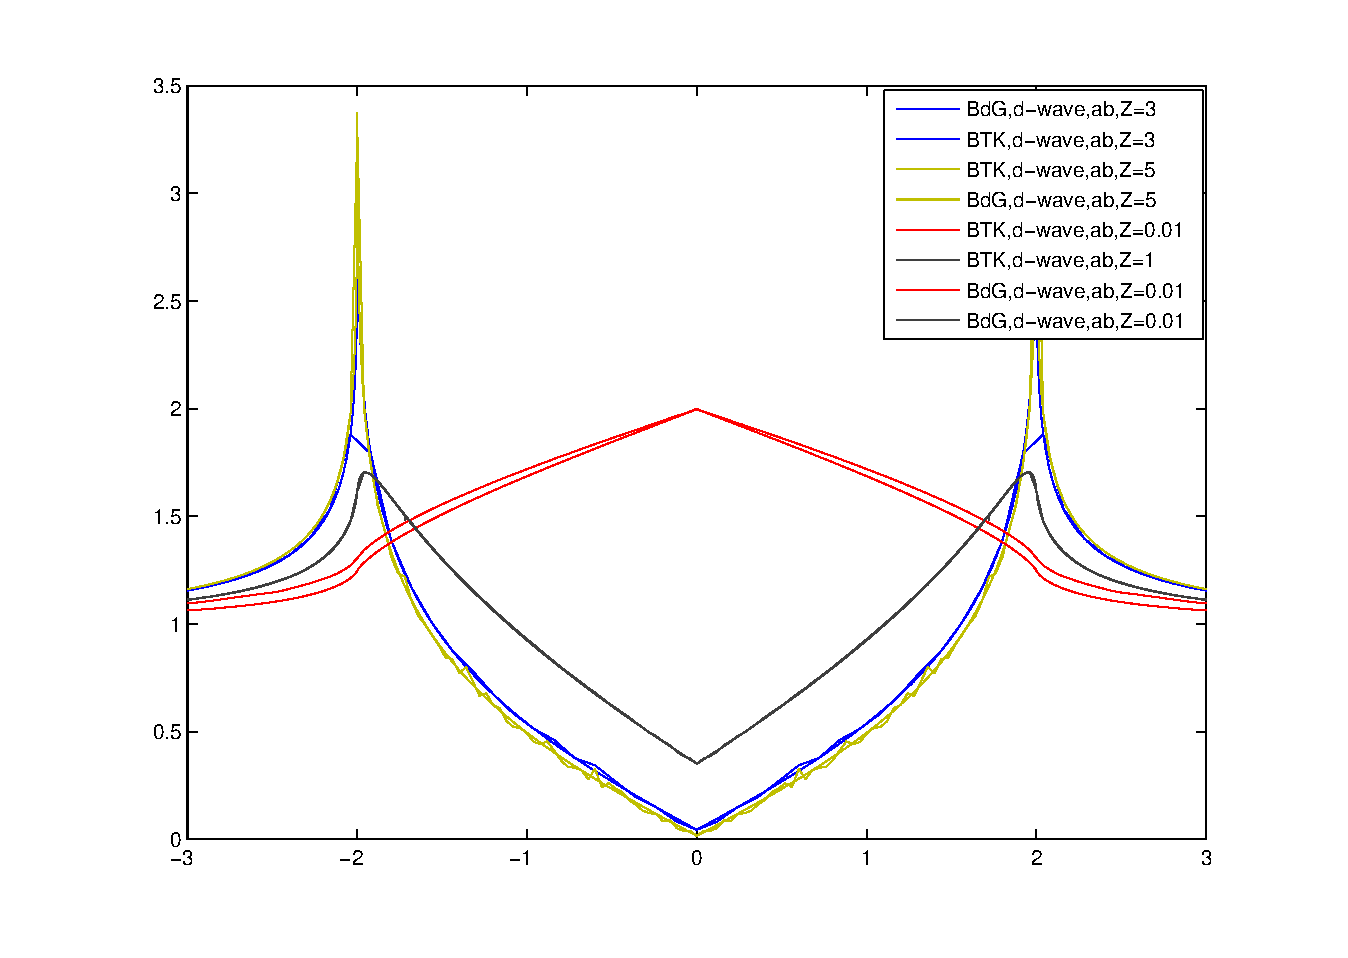
\includegraphics[width=8cm]{./Figures/BdGdwaveab.eps}
		\rule{35em}{0.5pt}
	\caption[An Electron]{The reproduction for the $d_{x^2-y^2}$ $ab$-tunnelling case. $Z_0=0.01,1,3,5$}
	\label{BdGdwaveab}
\end{figure}

In $c$-axis tunnelling in which we are more interested, we set pair potential as
\begin{eqnarray}\label{c momentum position}
\Delta(\varphi,z)=|\Delta(z)\cos2\varphi|
\end{eqnarray}
It can be derived from \eqref{General Energy Gap}. 
\begin{figure}[htbp]
\small
	\centering
		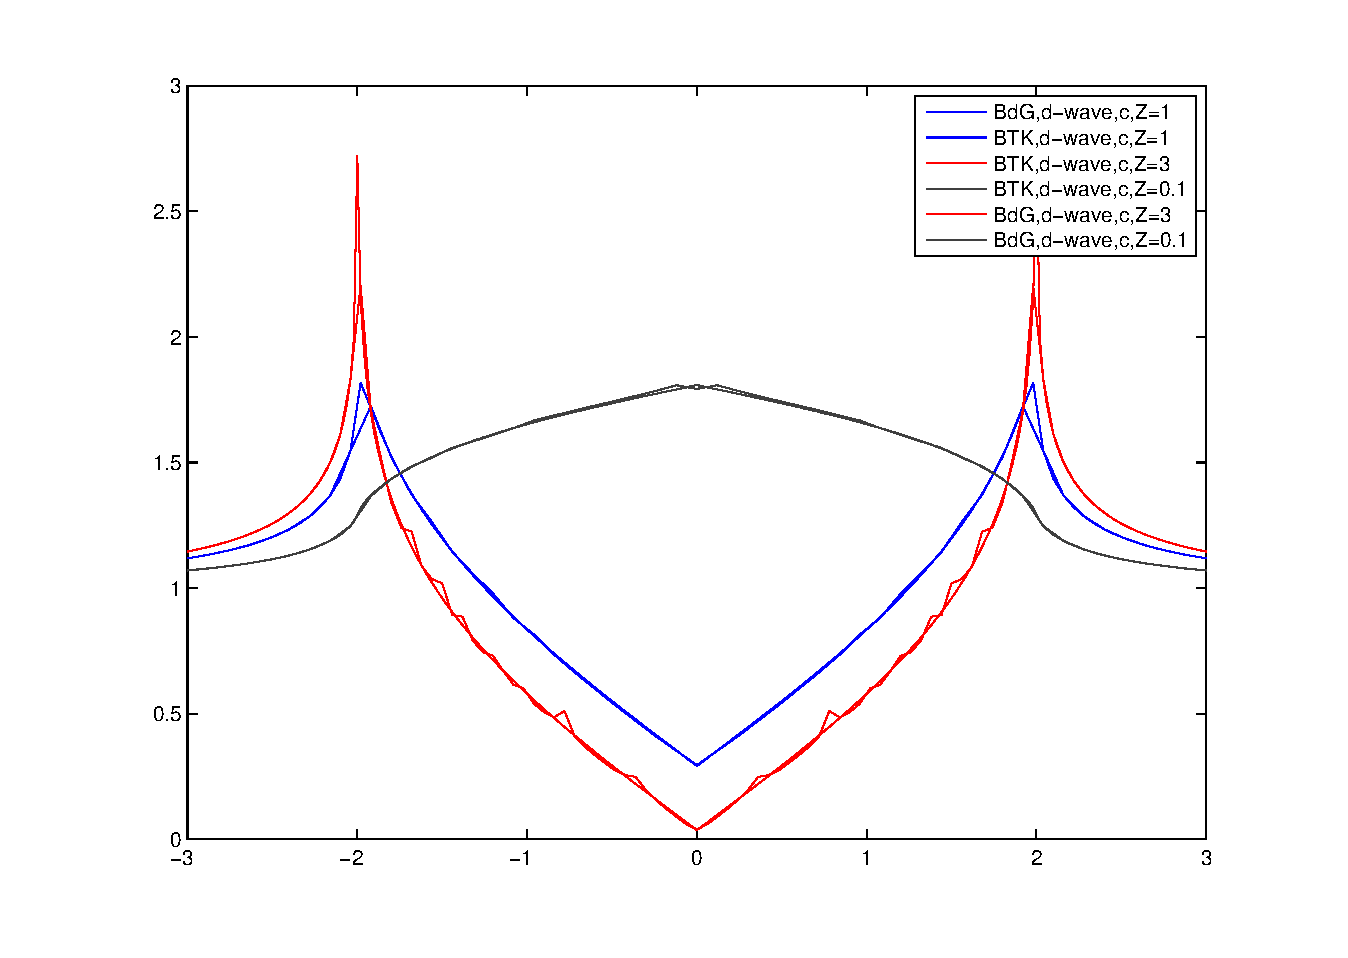
\includegraphics[width=8cm]{./Figures/Dcz.eps}
		\rule{35em}{0.5pt}
	\caption[An Electron]{The reproduction for the $d_{x^2-y^2}$ $c$-tunnelling case. $Z_0=0.1,1,3$}
	\label{Dcz}
\end{figure}
In Fig.\ref{Dcz}, we could see that the reproduction is fine.

We are still working on the $d$-wave proximity tunnelling spectroscopy. We did a trial calculation for the $d$-wave $ab$-tunnelling case. In the calculation, the $\cos\theta$ in \eqref{d wave BdG} is no longer trivial. Also, we can draw the conclusion from \eqref{d wave BdG} that if tunnelling at large incident angle, close to $\pm\pi/2$, the functions $u(z),v(z)$ will oscillate heavily. Meanwhile, $\cos\theta$ in the integral formula \eqref{2D-Kernel-Integral} is relatively small, in the light of which we do not have to do a complete half sphere integration, but within the domain $\theta\in[-1.5,1.5]$, so that a faster computation might be performed.
Fig.\ref{dabfull2-1-0.4} shows the proximity tunnelling conductance, the induced gap is clearly identified by the bulk in the centre. And the reduced gap is indicated by the second peak whose value, however is slightly larger than the reduced gap value. Also, as the figure is plotted in low resolution, we see some unwanted peaks around the bulk gap. Or it might be caused by the resonance due to thick proximity domain.  Fig.\ref{dabfullfull} shows the proximity tunnelling conductance with various reduced gaps and induced gaps. We can observe that with the same induced gap, the plots share the same bulk in the middle, similar to the figures of normal incident kernel Fig.\ref{Z=0.3reducedthin}-Fig.\ref{Z=0.3induced}. Fig.\ref{dabfullfull} shows additional plots for comparison.
\begin{figure}[htbp]
\small
	\centering
		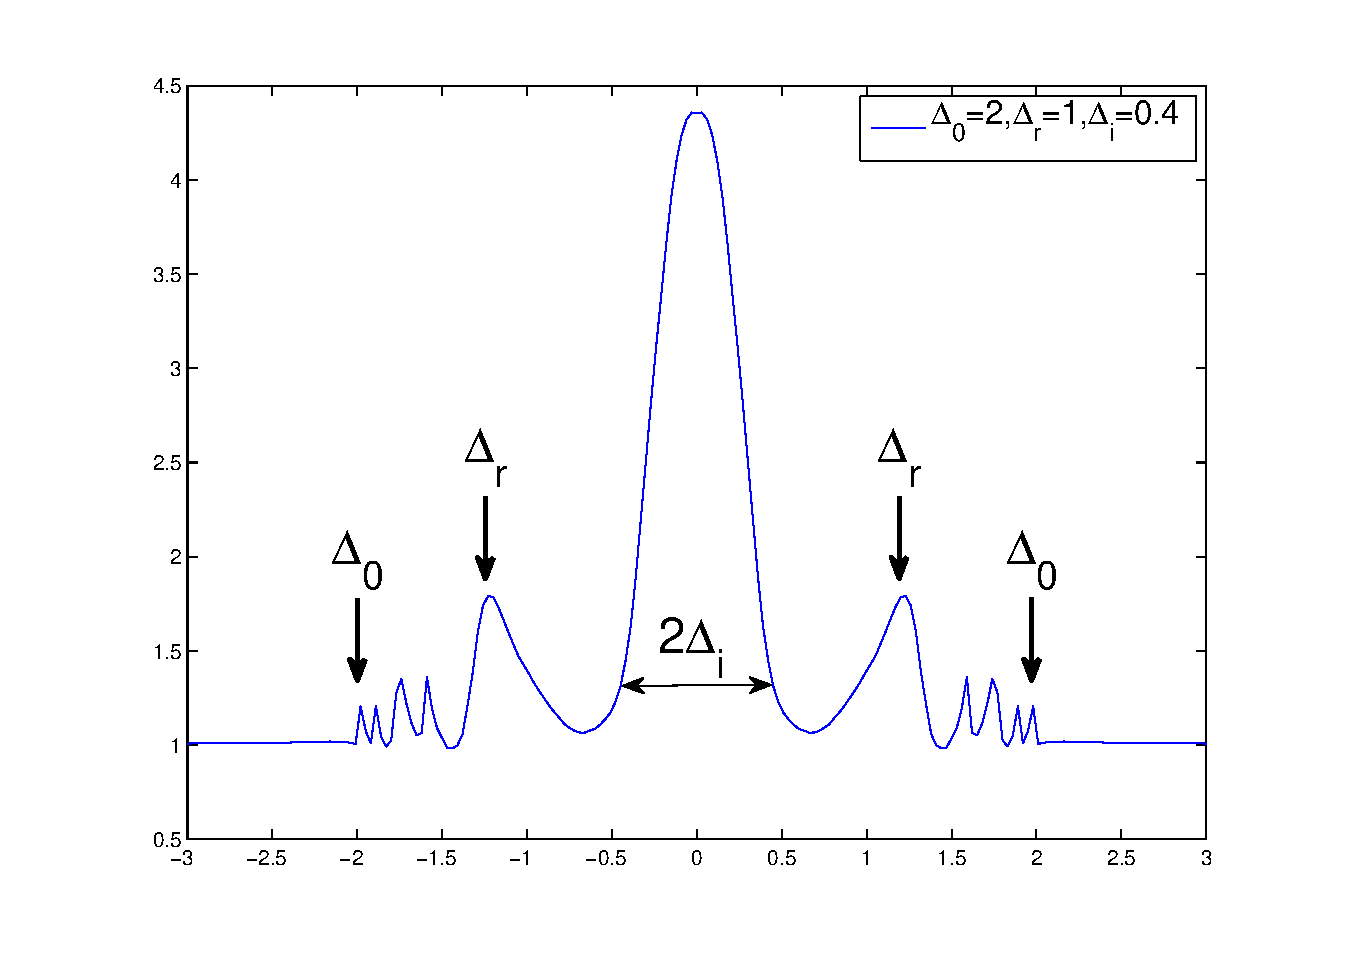
\includegraphics[width=8cm]{./Figures/fulldab2104.eps}
		\rule{35em}{0.5pt}
	\caption[An Electron]{The tunnelling conductance with bulk gap $\Delta_0=2$, reduced gap $\Delta_r=1$, $\Delta_i=0.4$, which are indicated in the figure. We can see that at the bulk gap side there are some oscillations, which may be due to the resolution of the calculation. $Z_0=1$}
	\label{dabfull2-1-0.4}
\end{figure}
\begin{figure}[htbp]
\small
	\centering
		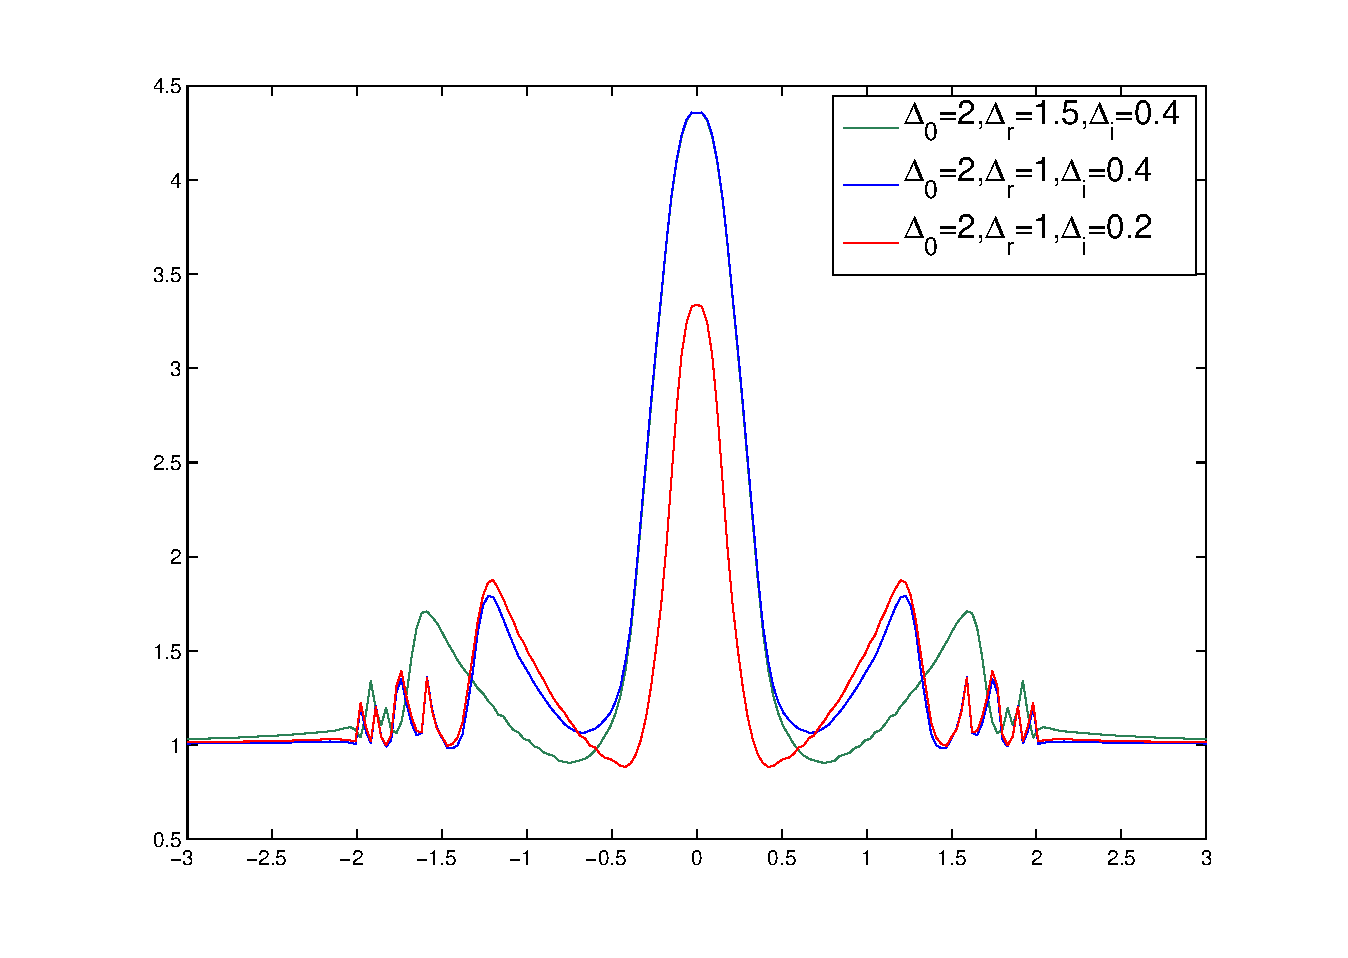
\includegraphics[width=8cm]{./Figures/fulldabfull.eps}
		\rule{35em}{0.5pt}
	\caption[An Electron]{The tunnelling conductance with various reduced gaps and induced gaps. $Z_0=1$.}
	\label{dabfullfull}
\end{figure}

Now we approach the $d$-wave $c$-tunnelling conductance. Similar to the case of $ab$-tunnelling, we conduct the integration within the domain $\varphi\in[0,2\pi], \theta\in[0,1.5]$. Fig.\ref{dcnewsingle} shows the proximity tunnelling conductance, the induced gap is clearly identified by the bulk in the centre. And the reduced gap is indicated by the second peak whose value, however is slightly larger than the reduced gap value. The shape of $c$-tunnelling conductance is quite similar to that of $ab$-tunnelling. Fig.\ref{dcnewfull} shows additional plots for comparison.
\begin{figure}[htbp]
\small
	\centering
		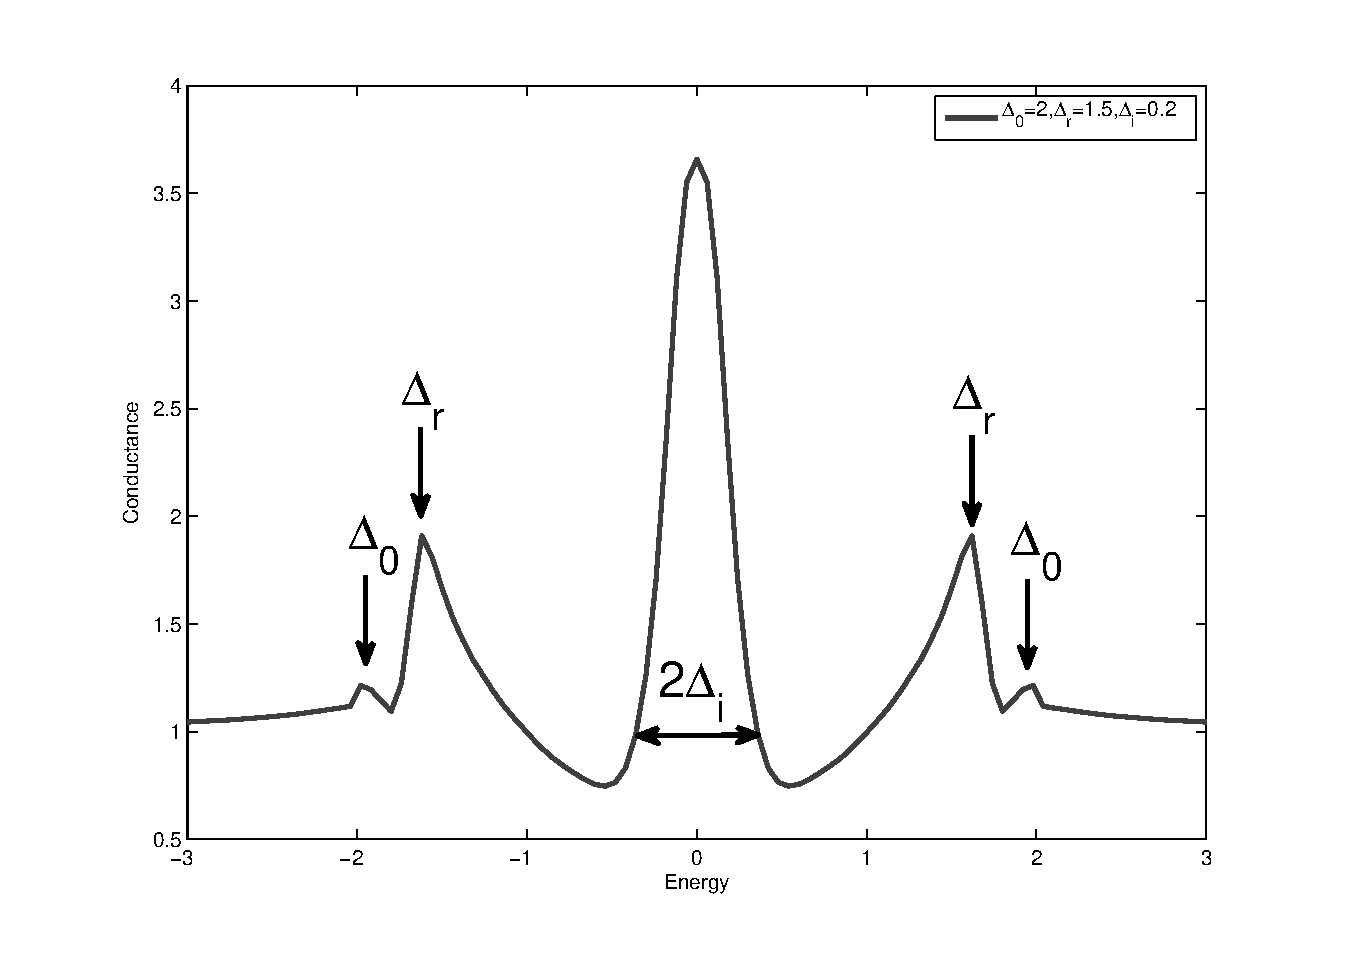
\includegraphics[width=8cm]{./Figures/dcnewsingle.eps}
		\rule{35em}{0.5pt}
	\caption[An Electron]{The tunnelling conductance with bulk gap $\Delta_0=2$, reduced gap $\Delta_r=1.5$, $\Delta_i=0.2$, which are indicated in the figure. $Z_0=1$}
	\label{dcnewsingle}
\end{figure}
\begin{figure}[htbp]
\small
	\centering
		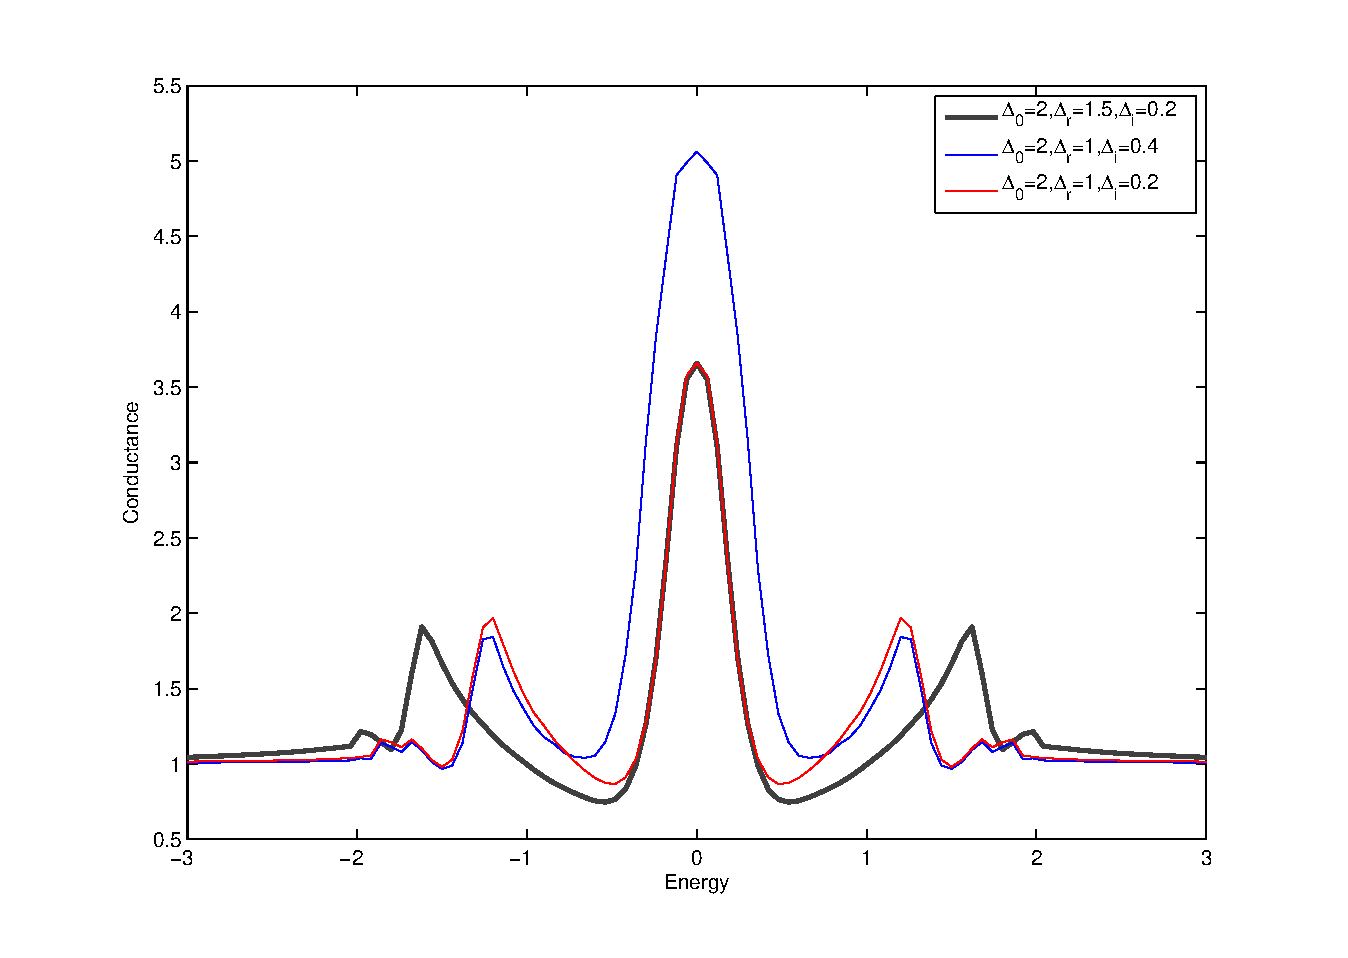
\includegraphics[width=8cm]{./Figures/dcnewfull.eps}
		\rule{35em}{0.5pt}
	\caption[An Electron]{The tunnelling conductance with various reduced gaps and induced gaps. $Z_0=1$.}
	\label{dcnewfull}
\end{figure}

























